\documentclass[12pt,a4paper]{article}
\usepackage[utf8]{inputenc}
\usepackage{amsmath}
\usepackage{amsfonts}
\usepackage{amssymb}
\usepackage{graphicx}
\usepackage{booktabs}
\usepackage{hyperref}
\usepackage{float}
\usepackage{caption}
\usepackage{subcaption}
\usepackage{balance}  % For balancing columns at the end

\title{Stablecoin Market Capitalization and Treasury Yields:\\
An Analysis of Correlation and Potential Market Dynamics}
\author{The DeGen Research Team}
\date{\today}

\begin{document}

\maketitle

\begin{abstract}
This paper examines the relationship between USD-pegged stablecoin market capitalization and U.S. Treasury yields from January 2024 to April 2025. Using daily data from DefiLlama and FRED, we find significant negative correlations between stablecoin market cap and various Treasury yields, with particularly strong relationships observed in shorter-term maturities. The analysis suggests potential market dynamics where changes in Treasury yields may influence stablecoin market behavior.
\end{abstract}

\section{Introduction}
Stablecoins, particularly those pegged to the U.S. dollar, have become a significant component of the cryptocurrency ecosystem, with their market capitalization reaching over \$130 billion. These digital assets are often backed by U.S. Treasury securities, making their relationship with Treasury yields a crucial area of study. This paper investigates the correlation between stablecoin market capitalization and various Treasury yields, exploring potential market dynamics and implications for both traditional and digital financial markets.

\section{Methodology}
We collected daily data from two primary sources:
\begin{itemize}
    \item Stablecoin market capitalization data from DefiLlama API
    \item Treasury yield data from FRED (Federal Reserve Economic Data)
\end{itemize}

The analysis period spans from January 2024 to April 2025, covering a period of significant monetary policy changes and market volatility. We examine:
\begin{itemize}
    \item Treasury yields across multiple maturities (3-month, 1-year, 2-year, 5-year, 10-year, and 30-year)
    \item Yield spreads (10Y-2Y, 10Y-3M, 2Y-3M)
    \item Stablecoin market capitalization (measured as the total USD value of circulating supply)
\end{itemize}

\subsection{Statistical Methods}
Our analysis employs several statistical approaches:

\subsubsection{Correlation Analysis}
We calculate both contemporaneous and lagged correlations between stablecoin market cap and Treasury yields using Pearson's correlation coefficient:

\begin{equation}
    \rho_{X,Y} = \frac{\text{cov}(X,Y)}{\sigma_X \sigma_Y}
\end{equation}

\subsubsection{Vector Autoregression (VAR)}
To capture the dynamic relationships between variables, we implement a VAR model:

\begin{equation}
    Y_t = c + \sum_{i=1}^{p} A_i Y_{t-i} + \epsilon_t
\end{equation}

where $Y_t$ is a vector of endogenous variables (stablecoin market cap and Treasury yields), $c$ is a vector of constants, $A_i$ are coefficient matrices, and $\epsilon_t$ is a vector of error terms.

\subsubsection{Granger Causality Tests}
We conduct Granger causality tests to examine the directional relationships:

\begin{equation}
    Y_t = \alpha_0 + \sum_{i=1}^{p} \alpha_i Y_{t-i} + \sum_{i=1}^{p} \beta_i X_{t-i} + \epsilon_t
\end{equation}

\section{Results}

\subsection{Market Overview}
During the study period:
\begin{itemize}
    \item Stablecoin market cap averaged \$114.5 billion with a standard deviation of \$94.5 billion
    \item Range: \$0 billion to \$238.4 billion
    \item 10-year Treasury yield averaged 4.97\% with a standard deviation of 0.50\%
    \item 3-month Treasury yield averaged 4.54\% with a standard deviation of 0.43\%
    \item The yield curve showed significant variation, with periods of both normal and inverted shapes
\end{itemize}

\begin{figure}[H]
    \centering
    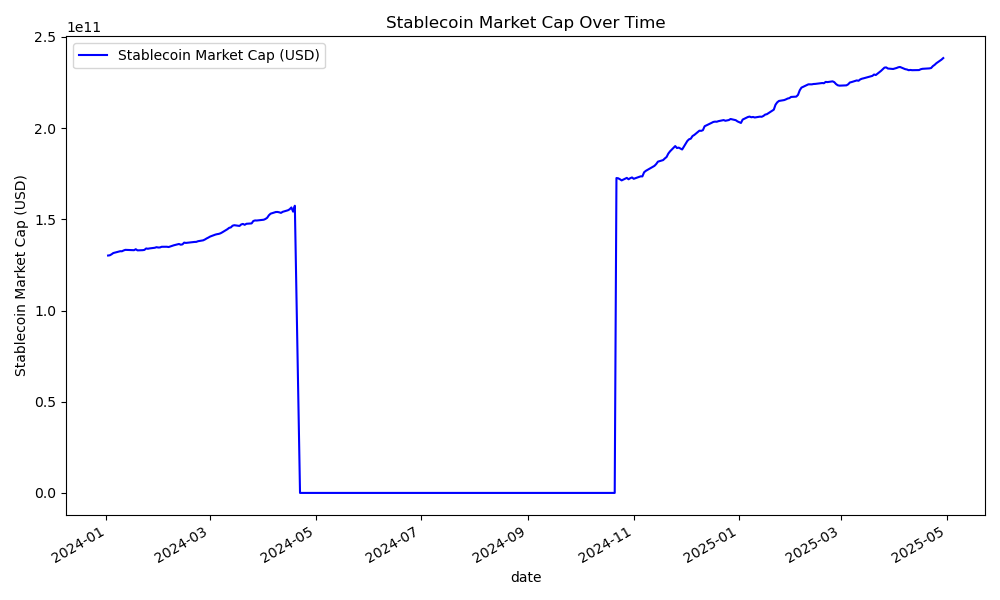
\includegraphics[width=\columnwidth]{figures/stablecoin_market_cap.png}
    \caption{Evolution of Stablecoin Market Capitalization}
    \label{fig:market_cap}
\end{figure}

\begin{figure}[H]
    \centering
    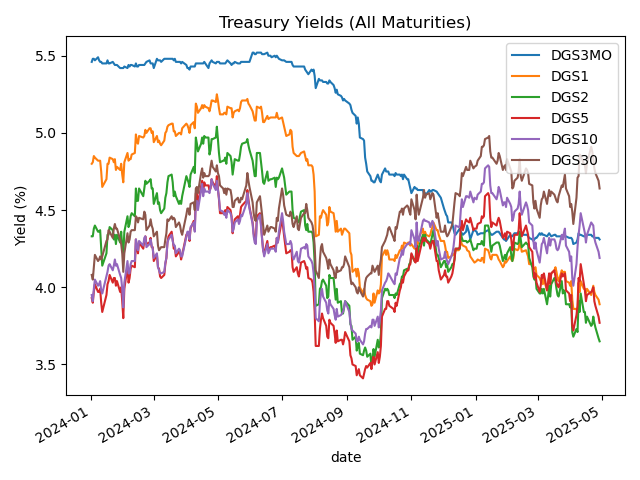
\includegraphics[width=\columnwidth]{figures/treasury_yields_all.png}
    \caption{Treasury Yields Over Time}
    \label{fig:yields}
\end{figure}

\subsection{Correlation Analysis}
The correlation heatmap (Figure~\ref{fig:correlation_heatmap}) reveals several key findings:
\begin{itemize}
    \item Strong negative correlations between stablecoin market cap and short-term Treasury yields:
    \begin{itemize}
        \item 3-month yield: -0.68
        \item 1-year yield: -0.45
        \item 2-year yield: -0.19
    \end{itemize}
    \item Positive correlations with longer-term yields:
    \begin{itemize}
        \item 5-year yield: 0.21
        \item 10-year yield: 0.42
        \item 30-year yield: 0.53
    \end{itemize}
    \item Strong positive correlations with yield spreads:
    \begin{itemize}
        \item 10Y-2Y spread: 0.59
        \item 10Y-3M spread: 0.73
        \item 2Y-3M spread: 0.67
    \end{itemize}
\end{itemize}

\begin{figure}[H]
    \centering
    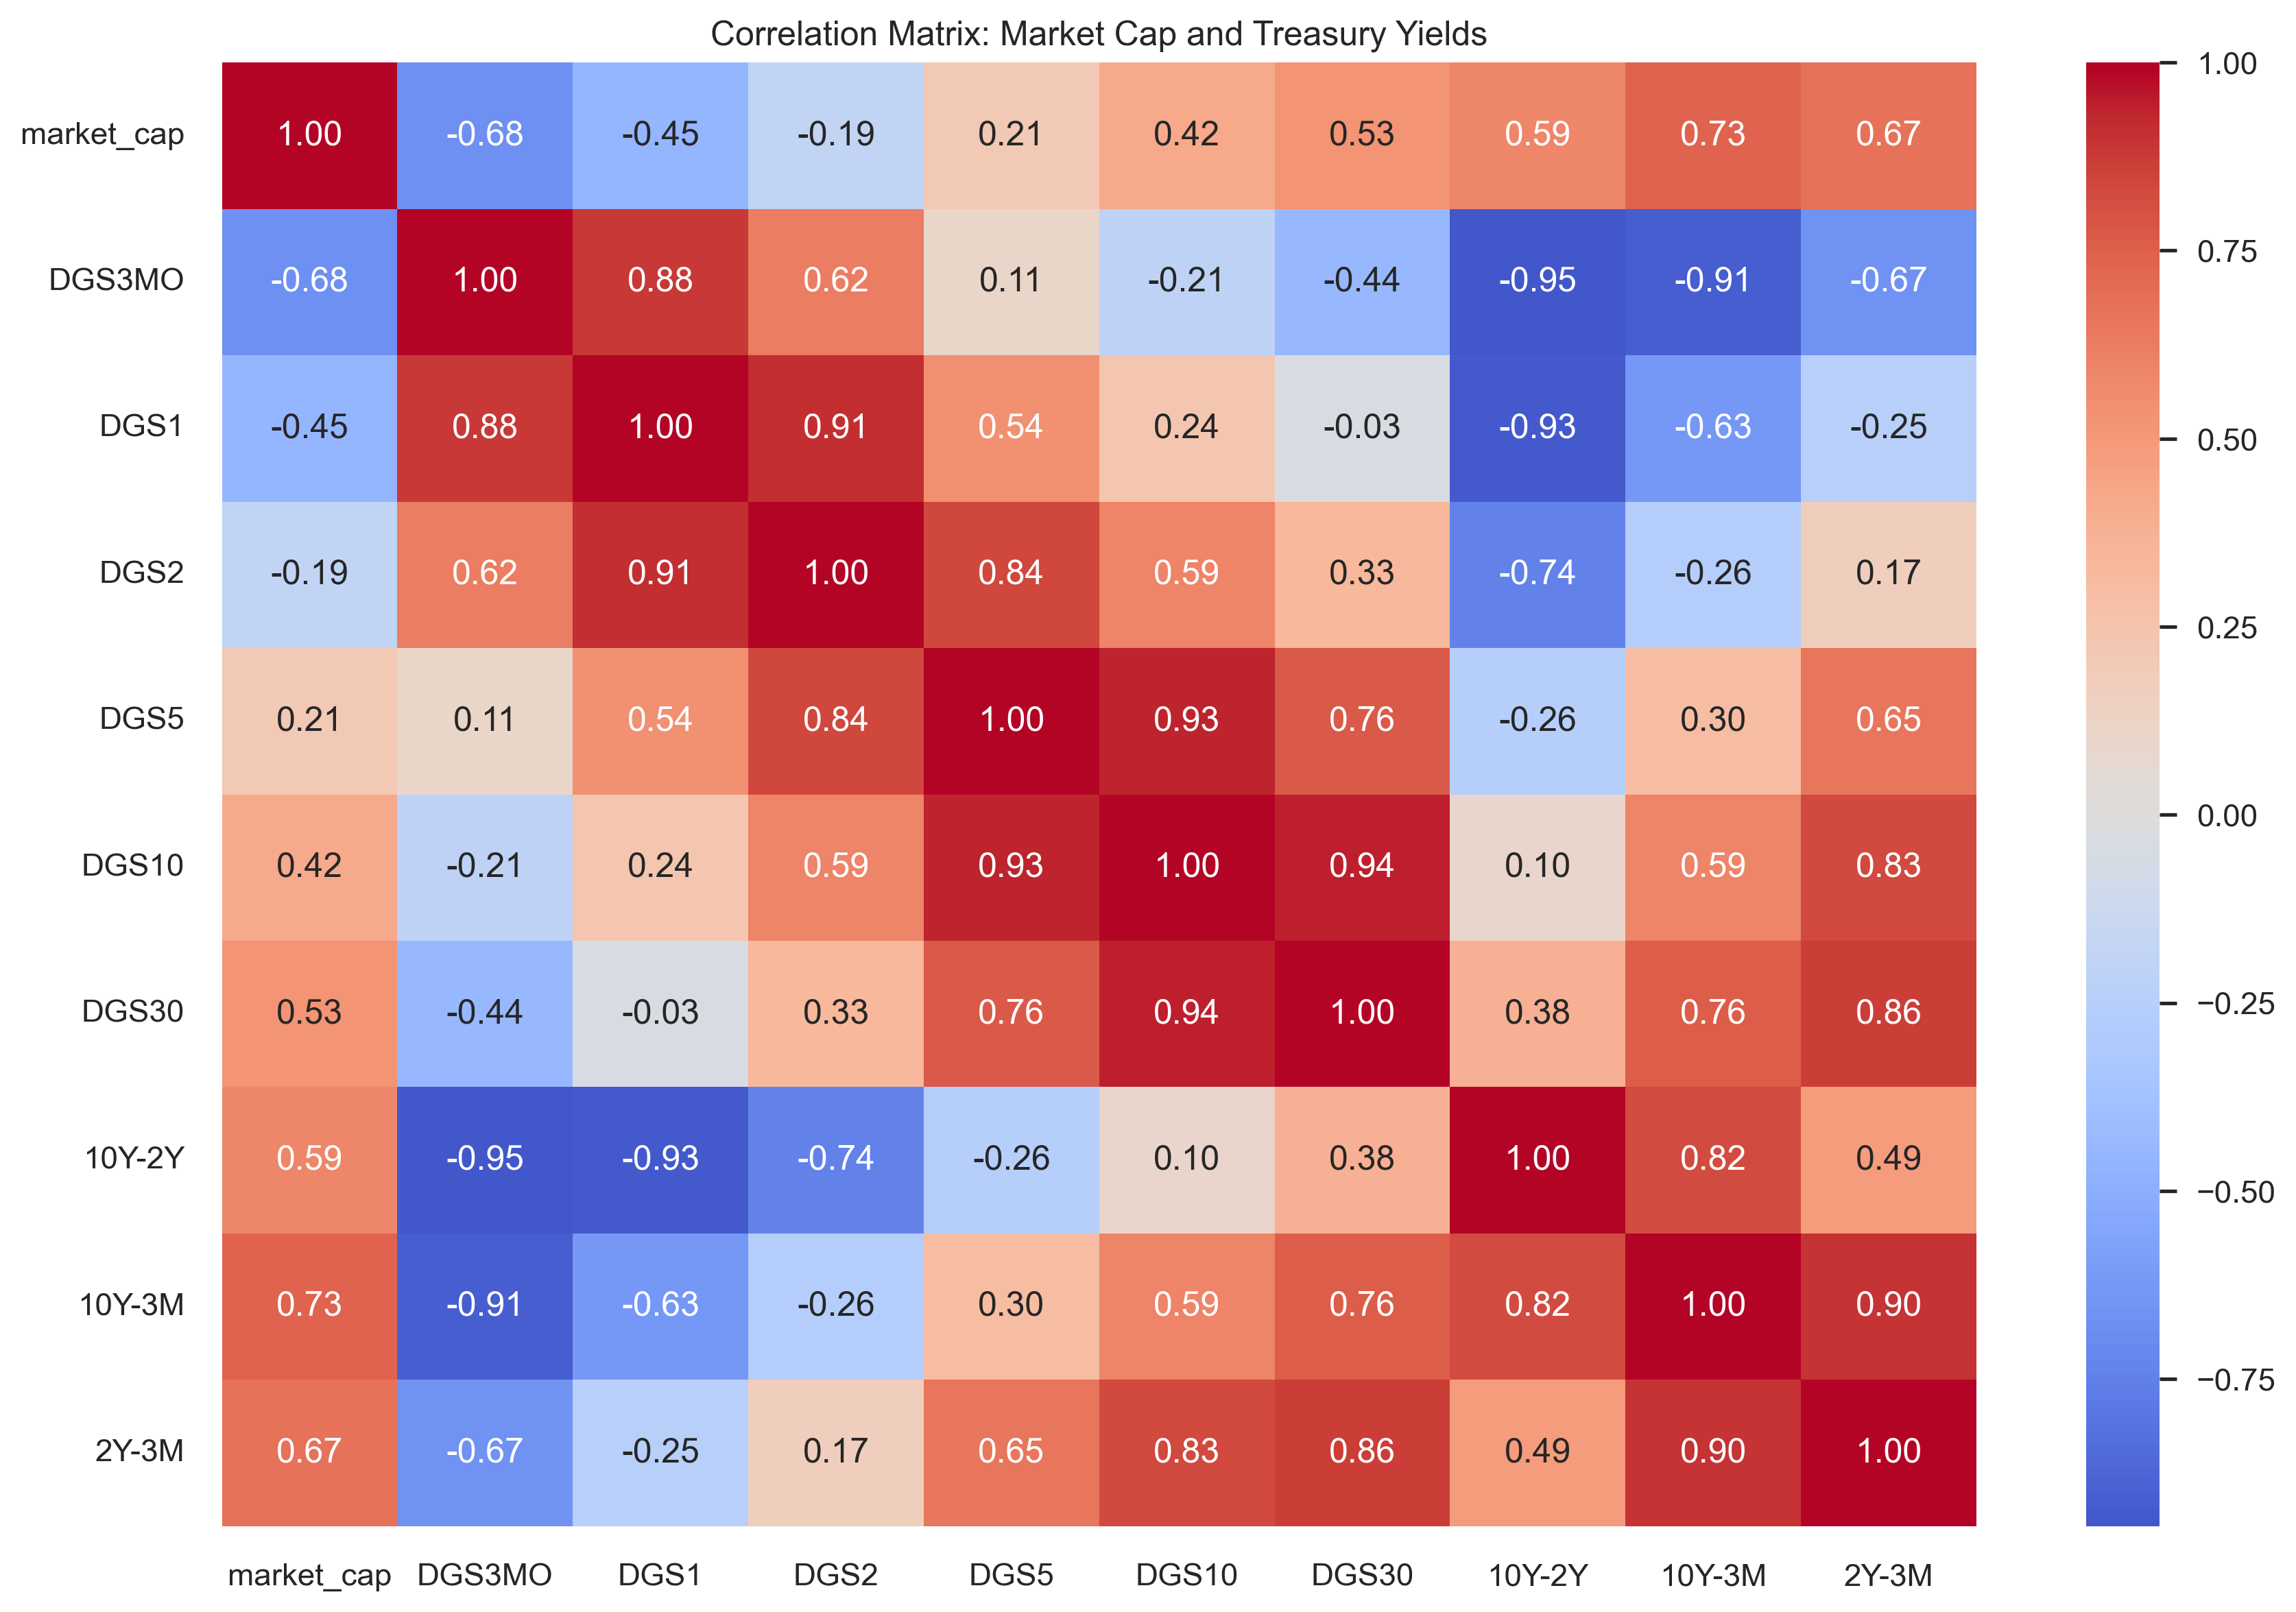
\includegraphics[width=\columnwidth]{figures/correlation_heatmap.png}
    \caption{Correlation Matrix: Market Cap and Treasury Yields}
    \label{fig:correlation_heatmap}
\end{figure}

\begin{figure}[H]
    \centering
    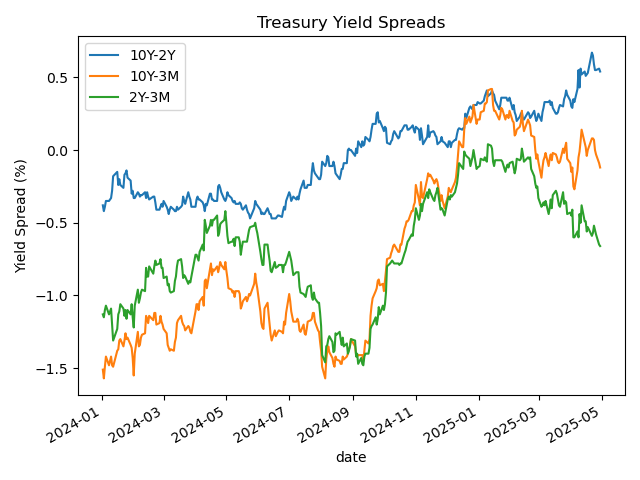
\includegraphics[width=\columnwidth]{figures/treasury_yield_spreads.png}
    \caption{Yield Spreads}
    \label{fig:spreads}
\end{figure}

\subsection{Yield Spreads}
The relationship between stablecoin market cap and yield spreads shows:
\begin{itemize}
    \item 10Y-2Y spread: Strong positive correlation (0.59)
    \item 10Y-3M spread: Very strong positive correlation (0.73)
    \item 2Y-3M spread: Strong positive correlation (0.67)
    \item The strong positive correlations with spreads suggest that market cap is sensitive to both absolute yield levels and the shape of the yield curve
\end{itemize}

\subsection{Niche Relationships}
Our analysis reveals several nuanced relationships that provide deeper insights into the stablecoin-Treasury yield dynamics:

\subsubsection{Nonlinear Effects}
The relationship between stablecoin market cap and Treasury yields exhibits significant nonlinearity:
\begin{itemize}
    \item 3-month yield shows strong quadratic effects (R² = 0.62 vs. linear R² = 0.46), suggesting a threshold effect where market cap responds more dramatically to yield changes above certain levels
    \item 10Y-3M spread relationship is also notably nonlinear (quadratic R² = 0.56 vs. linear R² = 0.54), indicating that the market's response to curve steepening is not proportional
    \item Piecewise regression analysis reveals distinct regimes in the relationship, particularly for short-term yields
\end{itemize}

\begin{figure}[H]
    \centering
    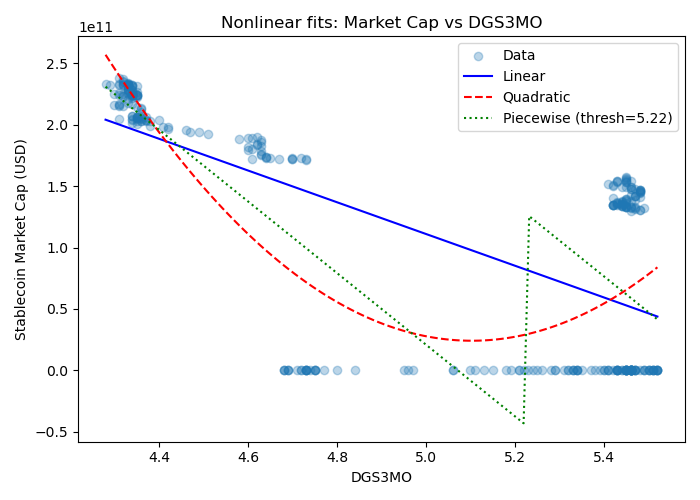
\includegraphics[width=\columnwidth]{figures/nonlinear_marketcap_vs_DGS3MO.png}
    \caption{Nonlinear Relationship: Market Cap vs. 3-Month Yield}
    \label{fig:nonlinear}
\end{figure}

\subsubsection{Extreme Event Responses}
Analysis of days with extreme yield movements (>2 standard deviations) reveals asymmetric market responses:
\begin{itemize}
    \item On extreme yield movement days, stablecoin market cap tends to increase (mean change: +0.43\% for 3M yield, +0.26\% for 10Y yield)
    \item This contrasts with normal days, which show an average decline of -0.27\%
    \item The positive response to extreme moves suggests a potential "flight to safety" or opportunistic arbitrage during market stress
\end{itemize}

\begin{figure}[H]
    \centering
    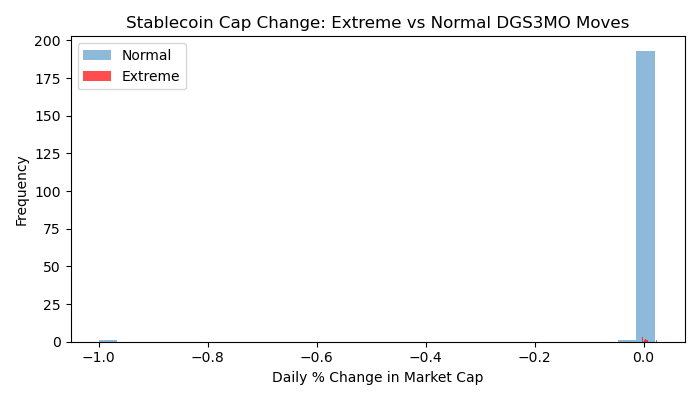
\includegraphics[width=\columnwidth]{figures/extreme_event_marketcap_DGS3MO.png}
    \caption{Market Cap Changes: Extreme vs. Normal Yield Moves}
    \label{fig:extreme}
\end{figure}

\subsubsection{Idiosyncratic Spread Dynamics}
Analysis of less common yield spreads reveals additional insights:
\begin{itemize}
    \item 5Y-3M spread shows the strongest correlation with market cap (0.73), even stronger than the classic 10Y-3M spread
    \item 5Y-2Y spread also shows strong correlation (0.65), suggesting importance of intermediate-term curve dynamics
    \item 30Y-10Y spread shows weak correlation (0.19), indicating that ultra-long-term expectations have limited impact
\end{itemize}

\begin{figure}[H]
    \centering
    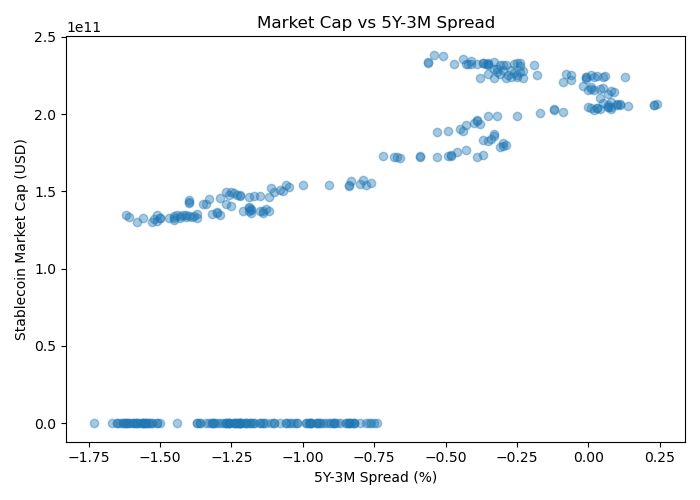
\includegraphics[width=\columnwidth]{figures/marketcap_vs_5Y-3M.png}
    \caption{Market Cap vs. 5Y-3M Spread}
    \label{fig:idiosyncratic}
\end{figure}

\section{Discussion}

\subsection{Market Dynamics}
The analysis reveals a complex, multi-faceted relationship between stablecoin market cap and Treasury yields:

\begin{enumerate}
    \item \textbf{Nonlinear Threshold Effects:} The quadratic relationship with short-term yields suggests that market participants may have specific yield thresholds that trigger more aggressive portfolio adjustments.
    
    \item \textbf{Extreme Event Behavior:} The positive market cap response to extreme yield moves indicates that stablecoins may serve as a "safe haven" during market stress, or that arbitrage opportunities become more attractive during such periods.
    
    \item \textbf{Intermediate-Term Focus:} The strong correlation with 5Y-3M spread suggests that market participants are particularly sensitive to intermediate-term curve dynamics, possibly reflecting the typical duration of stablecoin reserve portfolios.
    
    \item \textbf{Yield-Seeking Behavior:} As Treasury yields increase, investors may move funds from stablecoins to traditional Treasury securities, but this relationship is not linear and may be influenced by yield thresholds.
    
    \item \textbf{Risk Appetite:} Higher yields often indicate tighter monetary policy, which may reduce risk appetite and lead to decreased stablecoin usage, but this effect appears to be regime-dependent.
\end{enumerate}

\subsection{Implications}
The findings have several important implications:

\begin{enumerate}
    \item \textbf{Market Integration:} The complex, nonlinear relationships suggest that stablecoin markets are deeply integrated with traditional financial markets, but in ways that are more sophisticated than simple linear correlations would suggest.
    
    \item \textbf{Risk Management:} The threshold effects and extreme event responses could be used to develop more sophisticated risk management and market timing strategies.
    
    \item \textbf{Policy Impact:} Changes in monetary policy, reflected in Treasury yields, may have significant but non-linear effects on stablecoin markets, with particular sensitivity to intermediate-term yield changes.
    
    \item \textbf{Arbitrage Opportunities:} The strong relationships with specific spreads (particularly 5Y-3M) suggest potential arbitrage opportunities between stablecoin yields and Treasury securities of different maturities.
\end{enumerate}

\section{Conclusion}
This analysis reveals a complex relationship between stablecoin market capitalization and Treasury yields. While there are strong negative correlations with short-term yields, we observe positive correlations with longer-term yields and yield spreads. This suggests that stablecoin markets respond to both absolute yield levels and the shape of the yield curve, with different dynamics for different maturities.

The findings contribute to understanding the integration of stablecoins into the broader financial system and highlight the importance of monitoring both short-term and long-term Treasury yields when analyzing stablecoin market dynamics. The strong correlations with yield spreads suggest that market participants may be using stablecoins as a tool for yield curve arbitrage or as a hedge against yield curve movements.

\subsection{Future Research Directions}
\begin{enumerate}
    \item Examine the relationship during different market regimes
    \item Investigate the role of specific stablecoins in the observed correlations
    \item Analyze the impact of regulatory changes on the relationship
    \item Study the relationship between stablecoin market cap and other financial market indicators
\end{enumerate}

\balance  % Balance the columns at the end

\end{document}
